\subsection{Terrain Generator}
\begin{center}
  \textit{User parameters} $\rightarrow$ \textbf{TerrainGenerator}  $\rightarrow$ \textit{Terrain}
\end{center}

We will approach this subproblem by first generating a heightmap that represents the hills and the valleys of the terrain.
A heightmap is a bitmap image where each pixel typically store values representing a surface elevation or displacement.
This is often visualized as a grayscale image where the black pixels represents the minimum elevation, and white represents the maximum elevation.
For this project's particular use case the pixel values will store the terrain elevations, which will be rendered as a 3D mesh.
One limitation of using heightmaps is that they can not represent more complex 3D geometry such as caves or overhangs.
However since the main focus of the project is on procedurally generating cities, and not terrain, this is not regarded as a problem.
Figure~\ref{fig:heightmap} illustrates an example heightmap visualized as a grayscale image.

% NOTE(anton): image generated from https://cpetry.github.io/TextureGenerator-Online/
\begin{figure}[h]
  \centering
  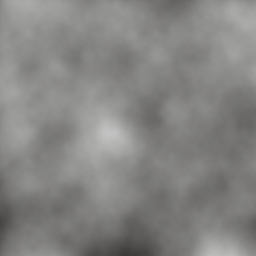
\includegraphics[width=0.25\textwidth]{figure/heightmap.png}
  \caption{An example heightmap generated using Perlin Noise.}
  \label{fig:heightmap}
\end{figure}

We plan to generate the heightmap using multiple layers of simplex noise.
Each octave, or layer, of simplex noise will represent different levels of terrain granularity.
Higher frequency of noise corresponds to an area on the heightmap where we would like to generate an area with a small, yet intense difference in elevation.
Whereas lower frequencies will correspond to areas of a less intense, but larger difference in elevation forming the contour of the terrain.
This can be used to generate both smooth hills and rocky mountains.

The color of the terrain will be based on the height levels e.g.\ grasslands near sea level, rocky mountain textures for the taller regions, and snow for top peaks of some of the taller mountains.
One approach for achieving this is a technique called Texture splatting that is commonly used for terrain rendering.
This method consists of combining different textures blended together according to an alphamap, also referred to as a weightmap or splatmap.
Figure~\ref{fig:texture-splatting} demonstrates this technique in action.

\begin{figure}[H]
  \centering
  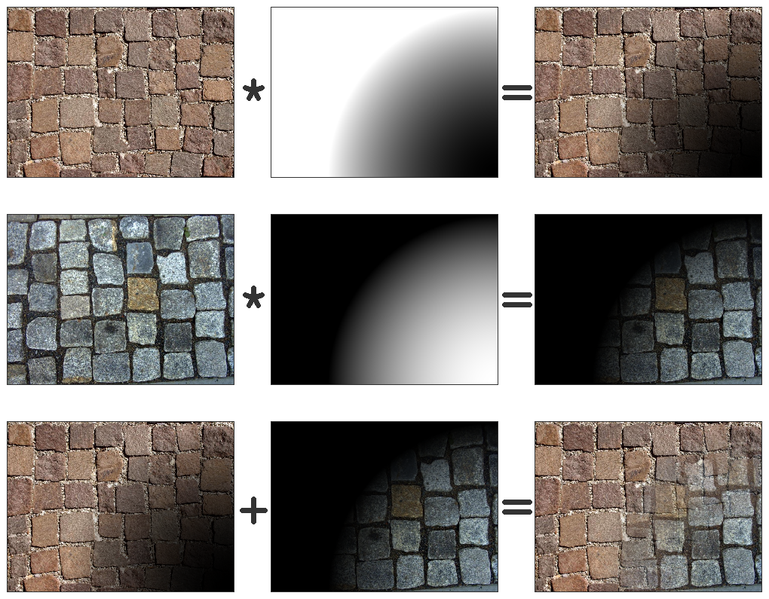
\includegraphics[width=0.4\textwidth]{figure/texture-splatting.png}
  \caption{Example of texture splatting from related work \cite{wiki:texture-splatting-img}}
  \label{fig:texture-splatting}
\end{figure}

Furthermore the user can provide a threshold height for the sea level where any point of the terrain below this threshold value will be filled with ocean. 
This can simply be done with drawing an animated water texture on a plane positioned at said height level. 

As previously mentioned in the problem section, there are some things that could be added to our project in the later stages, if there is time for them. 
We could for example add water flowing from mountains that turns into rivers, and similarly we could make these rivers flow into lakes in order to make our terrain look more natural.
For now we have only speculated on how we would like to approach this problem, but we have discussed forming rivers using a gradient descent starting from the mountain-tops.
The way a river flows would be determined by \textit{river agents} based on the gradient descent function from mountain-top to ground level. 
We could then decide to, depending on where the river agent \textit{terminates}  to perform different actions on that part of the terrain.
If a river flows into the ocean we would not need to create anything, but if a river flows into seemingly nothing we could decide to generate a lake there. 

Another approach would be to generate the lakes seemingly arbitrary at first, and then try to find a gradient descent path from the mountain-tops to the lakes.
If no such paths are found, we do nothing, but if the agents finds a path we generate a river from the mountain to the lake. 


